% \documentclass[handout]{beamer}
\documentclass{beamer}
\usetheme{Boadilla}

\usepackage{cancel}

\title[Physics Problem Solving]{From Brachistochrone Curve to Calculus of Variations}
\subtitle{How Understanding of Physics Evolve with Mathematics}
\author{Eason Shao}
\institute[]{Physics Problem Solving Society\\St Paul's School}
\date{24.06.2024}

\newcommand{\diff}{\mathsf{d}}

\begin{document}

\frame{\titlepage}

\begin{frame}{Table of Contents}
    \tableofcontents
\end{frame}

\section{Historical Overview}

\begin{frame}{History of Mathematics and Physics} \pause
    Mathematics and Physics are highly inter-correlated (but at the same time fundamentally different). \pause

    Their relationship can be split into three stages: \pause

    \begin{enumerate}
        \setcounter{enumi}{-1}

        \item Aristotle, Archimedes, ...: No particular relation. Physics was highly experimental and experience-based. \pause
        \item Newton: Vector Analysis (and Real Analysis/Calculus). \pause
        \item Euler, Lagrange: Functional Analysis (Calculus of Variations). \pause
        \item Noether: Symmetry (Group Theory and Modern Algebra). e.g., QFT, CPT, QED, QCD.
    \end{enumerate}
\end{frame}

\begin{frame}{Physics at Newton's Time}
    Newton's work: \pause
    \begin{itemize}
        \item \textit{Philosophiæ Naturalis Principia Mathematica}, 1687, gives rise to Classical Mechanics. \pause
        \item One of the first Mathematical Formulations of Physics. \pause
        \item Relies on the geometry of our space (being flat). \pause
        \item Kepler's Laws, elementary electromagnetism, and even elementary thermal physics can be described using forces and motion. \pause
    \end{itemize}

    Restrictions: \pause
    \begin{itemize}
        \item Highly relies on a straight-line motion, which restricts the degree of freedom. \pause
        \item Uses local linear behaviour to analyse complicated paths. \pause
        \item This makes thermodynamics highly inaccurate and unable to solve certain questions.
    \end{itemize}
\end{frame}

\begin{frame}{The Brachistochrone Curve Problem} \pause
    \textit{This question is related to the \textbf{Tautochrone Curve Problem} (which has the same solution).} \pause

    \begin{block}{Brachistochrone Curve Problem (Galilei, 1638 and Bernoulli, 1696)}
        What is the \textbf{Brachistochrone Curve}, or the curve of fastest descent, which is the one lying on the plane between a point \(A\) and a lower point \(B\) (where \(B\) is not directly below \(A\)) on which a bead slides frictionlessly under the influence of a uniform gravitational field along the curve from \(A\) to \(B\) in the shortest \textbf{time}?
    \end{block} \pause

    Please guess what the curve could be before we continue.
\end{frame}

\begin{frame}{History of the Problem}
    \begin{itemize}
        \item Galilei, 1638: Concluded that the arc of a circle is faster than any number of its chords and concluded incorrectly that the arc is the quickest \pause - but warned of possible fallacies and the need for a higher science. \pause
        \item Johann Bernoulli and Jakob Bernoulli, 1696: Derived the same conclusion (but Johann was incorrect). \pause They also realised this has the same solution as the Tautochrone Problem (Huygens). \pause
        \item Newton, 1697: Found the solution because he stayed up for a whole night and posted to Bernoulli.
    \end{itemize}
\end{frame}

\begin{frame}{Abstraction and Formulation} \pause
    To simplify the problem, we build a coordinate system where the origin is the starting point, the \(y\) axis points down, and the \(x\) axis points to the right. \pause Also, assume the ending point is \((a, b)\). \pause

    If we denote the curve as \(y = y(x)\), we must have boundary conditions \(y(0) = 0\) and \(y(a) = b\). \pause

    By conservation of energy, \pause we will have the speed \(v\) at a general point \((x, y)\) satisfies that
    \[
        \frac{1}{2}mv^2 = mgy \pause \implies v = \sqrt{2gy}.
    \] \pause

    Also, since \(v = \frac{\diff s}{\diff t}\), and by Pythagerous Theorem we have
    \[
        \diff s = \sqrt{\diff x^2 + \diff y^2} \pause = \diff x \sqrt{1 + \left(\frac{\diff y}{\diff x}\right)^2} \pause = \sqrt{1 + (y')^2} \diff x.
    \]
\end{frame}

\begin{frame}
    This means that
    \[
        v = \frac{\diff s}{\diff t} = \sqrt{1 + (y')^2} \frac{\diff x}{\diff t},
    \] \pause
    and hence
    \[
        \diff t = \sqrt\frac{1+(y')^2}{2gy} \diff x.
    \] \pause

    Therefore, the total time taken, \(T\), will satisfy that
    \[
        T = \int \diff t \pause = \int_{0}^{a} \sqrt \frac{1 +(y')^2}{2gy} \diff x = \frac{1}{\sqrt{2g}} \int_{0}^{a} \sqrt \frac{1 +(y')^2}{y} \diff x.
    \] \pause

    Our task is to find \(y\) that it minimises such \(T\).
\end{frame}

\section{Analytical Mechanics}

\begin{frame}{Functionals} \pause
    \begin{definition}[Functional]
        A function \(\mathcal{F}\) is called a functional if it takes in some function as its parameter and outputs a scalar value as its result.
    \end{definition} \pause

    \begin{examples}
        \begin{itemize}
            \item \(\mathcal{I}[f] = f(0)\) \pause is a functional \pause since it takes in a function \(f\) and outputs its value at \(0\). \pause
            \item \(\mathcal{J}[f] = \int_{0}^{1} f(x) \diff x\) \pause is a functional. \pause It outputs the area under the curve \(f(x)\) from \(x = 0\) to \(x = 1\). \pause
            \item \(\mathcal{K}[f] = \frac{\diff f}{\diff x}\) \pause is not a functional. \pause It does not output a scalar value.
        \end{itemize}
    \end{examples}
\end{frame}

\begin{frame}{Euler-Lagrange Equation} \pause
    \begin{theorem}[Euler-Lagrange Equation]
        A functional \(\mathcal{J}\) takes in a path \(y\) with the boundary conditions \(y(a) = A\) and \(y(b) = B\):
        \[
            \mathcal{J}[y] = \int_{a}^{b} L(x, y, y') \diff x,
        \]
        where \(L\) is some expression. \pause

        \(\mathcal{J}\) takes some extremum if and only if the equation
        \[
            \frac{\partial L}{\partial y} - \frac{\diff}{\diff x}\frac{\partial L}{\partial y'} = 0
        \]
        is satisfied.
    \end{theorem}
\end{frame}

\begin{frame}
    \begin{example}[Shortest Path]
        The length of a path \(y = y(x)\) between two points \((a, A)\) and \((b, B)\) is
        \[
            s = \int_{a}^{b} \sqrt{\diff x^2 + \diff y^2} = \int_{a}^{b} \sqrt{1 + (y')^2} \diff x.
        \] \pause

        The \(L\) in the equation is \(L(x, y, y') = \sqrt{1 + (y')^2}\). \pause

        We will realise that
        \[
            \frac{\partial L}{\partial y} = 0, \frac{\partial L}{\partial y'} = \frac{y'}{\sqrt{1 + (y')^2}}.
        \]
    \end{example}
\end{frame}

\begin{frame}
    \begin{example}[Shortest Path]
        \[
            \frac{\partial L}{\partial y} = 0, \frac{\partial L}{\partial y'} = \frac{y'}{\sqrt{1 + (y')^2}}.
        \]
        If we substitute this into the equation, we will get that \pause
        \[
            \frac{\diff}{\diff x} \frac{y'}{\sqrt{1 + (y')^2}} = 0,
        \] \pause
        and therefore
        \[
            \frac{y'}{\sqrt{1 + (y')^2}} = \text{const}.
        \] \pause
        This means that
        \[
            y' = \frac{\text{const}}{\sqrt{1 - \text{const}^2}} = \text{another const},
        \] \pause
        which means it is a straight line!
    \end{example}
\end{frame}

\begin{frame}{Solution of Problem}
    In the original problem, we would like to minimise
    \[
        T = \frac{1}{\sqrt{2g}} \int_{0}^{a} \sqrt \frac{1 +(y')^2}{y} \diff x.
    \] \pause

    Our \(L\) here is
    \[
        L(x, y, y') = \sqrt \frac{1 + (y')^2}{y}.
    \] \pause

    (If you trust my differentiation skills) We will have
    \[
        \frac{\partial L}{\partial y} = -\frac{1}{2} \sqrt\frac{1 + y'^2}{y^3}, \frac{\partial L}{\partial y'} = \frac{y'}{\sqrt{y (1 + y')^2}},
    \] \pause
    and plugging it back into the equation, mathematicians will tell us the solution is a cycloid.
\end{frame}

\begin{frame}{Visuallisation}
    A cycloid: \pause

    \begin{center}
        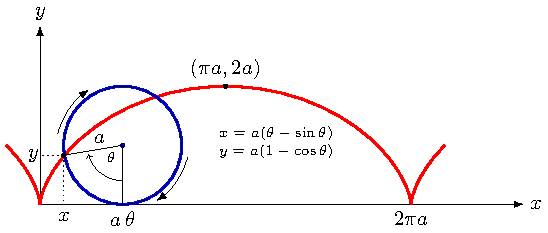
\includegraphics[scale=1.2]{cycloid.pdf}
    \end{center}

\end{frame}

\begin{frame}
    Different curves: \pause

    \begin{center}
        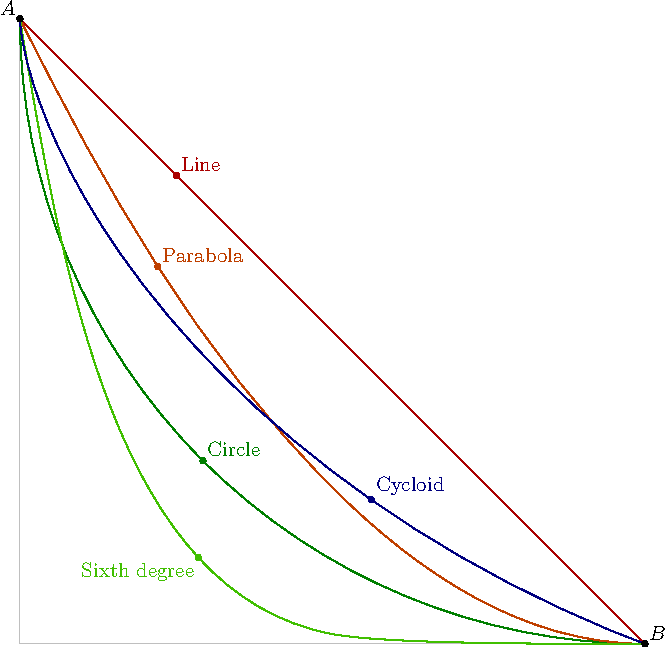
\includegraphics[scale=0.75]{compareCurve.pdf}
    \end{center}
\end{frame}

\begin{frame}{Calculus of Variations} \pause
    Calculus of Variations is the study of how we can minimise functionals by varying functions. \pause

    The idea is similar: \pause
    \begin{itemize}
        \item To minimise \(y = f(x)\), \pause we solve for \(f'(x) = 0\). \pause
        \item To minimise \(t = f(x, y, z)\), \pause we solve for \(\frac{\partial f}{\partial x} = \frac{\partial f}{\partial y}  = \frac{\partial f}{\partial z} = 0\). \pause
        \item To minimise \(\mathcal{L}[f]\), \pause we solve for the Euler-Lagrange equation, which generalises to Euler-Poisson Equation and others. \pause
    \end{itemize}

    The idea of variation of a function is by doing \(y (x) = y_0 (x) + \epsilon \eta (x)\) where \(\eta(x)\) is an arbitary fucntion and \(\epsilon \rightarrow 0\).
\end{frame}

\begin{frame}{Lagrangian and Hamiltonian Mechanics}
    \begin{align*}
        \mathcal{L} & = - \frac{1}{4} F_{\mu \nu} F^{\mu \nu}               \\
                    & \phantom{{}=}+ i \bar{\psi} \cancel{D} \psi + h.c.    \\
                    & \phantom{{}=}+ \bar{\psi}_i y_{ij} \psi_j \phi + h.c. \\
                    & \phantom{{}=}+ |D_\mu \phi|^2 - V(\phi)
    \end{align*} \pause
    is the Lagrangian of the standard model. \pause

    Doing something similar to (but much more complicated than) the Euler-Lagrange equation and solving it will enable you to explain everything apart from gravity. \pause

    Hamilton, 1833 provides an alternative formulation using the Hamiltonian \(\mathcal{H}\). \pause

    These will be covered next week by Dara Daneshvar - come if you are interested!
\end{frame}

\begin{frame}{Benefits}
    If we look back at our derivation of the solution: \pause
    \begin{itemize}
        \item we used energy rather than forces, \pause
        \item we used path rather than points, \pause
    \end{itemize}
    and we are considering an action along the path. \pause

    \begin{itemize}
        \item It does not assume any geometry of the space, and does not ignore interior structures of objects, does not use simple linear approximations. \pause
        \item It converts all problems to finding the extremum of some quantity - and applying variations to such quantity will enable us to form a sophisticated but self-consistent system. \pause
    \end{itemize}

    It provides a unified way to solve all kinds of different physical problems.
\end{frame}

\begin{frame}{Applications} \pause
    \begin{itemize}
        \item Direct applications in mechanics include the Principle of Least Action and Hamilton's Principle. \pause
        \item We can also apply variation to maximise entropy - or minimise free energy - in thermodynamics,  and they lead to the same result. \pause
        \item We can also apply variation on the Lagrangian density of an electromagnetic field to deduce Maxwell's Equations (and this even works for QED). \pause
        \item We can use calculus of variations to deduce Einstein's field equations based on Einstein-Hilbert action in general relativity.
    \end{itemize}
\end{frame}

\section{Restrictions}

\begin{frame}{Restrictions of this Mathematical Formulation}
    Mathematics should not rely on intuition, but Physics should, or at least an intuitive explanation should exist alongside an abstract formulation. \pause

    So what is
    \[
        L(x, y, y') = \sqrt \frac{1 + (y')^2}{y},
    \]
    and what is
    \[
        \frac{\partial L}{\partial y} - \frac{\diff}{\diff x}\frac{\partial L}{\partial y'} = 0?
    \] \pause

    What is action, what is entropy, what is free energy? \pause

    This is very much less intuitive than forces and speed in Newtonian Mechanics.
\end{frame}

\begin{frame}{Symmetry, Group Theory, and Noether's Theorem} \pause
    \begin{theorem}[Noether's Theorem]
        Every continuous symmetry of the action of a physical system with conservative forces has a corresponding conservation law.
    \end{theorem} \pause

    \begin{examples}
        \begin{itemize}
            \item Energy conserves since physical laws have time symmetry (i.e., physical laws do not change over time). \pause
            \item Momentum conserves since physical laws have space symmetry (i.e., physical laws do not change under translation).
        \end{itemize}
    \end{examples} \pause

    Under this formulation, the Lagrangian we see can simply take the mathematical structure of a group, specifically the group
    \[
        \mathsf{SU}(3) \times \mathsf{SU}(2) \times \mathsf{U}(1)
    \] \pause
    This is how Physics in the recent century developed.
\end{frame}

\begin{frame}
    \begin{quote}
        The chief forms of beauty are order and symmetry and definiteness, which the mathematical sciences demonstrate in a special degree.

        \hfill -- Aristotle
    \end{quote}
\end{frame}

\begin{frame}{Solving the Differential Equation}
    If we recall
    \[
        \frac{\partial L}{\partial y} = - \frac{1}{2} \sqrt\frac{1 + y'^2}{y^3}, \frac{\partial L}{\partial y'} = \frac{y'}{\sqrt{y(1+y')^2}},
    \]
    we can simplify the equation to\pause
    \[
        \frac{1}{2}(1 + y'^2) + y y'' = 0.
    \]
    
    If we multiply \(2y'\) on both sides,
    \[
        y'(1 + y'^2) + 2yy'y'' = 0 \pause \implies \frac{\diff}{\diff x} \left[y (1 + y'^2)\right] = 0.
    \]\pause

    This means that for some constant \(k\), we have
    \[
        y(1 + y'^2) = k \pause \implies y' = \frac{\diff y}{\diff x} = \sqrt\frac{k - y}{y}.
    \]
\end{frame}

\begin{frame}
    If we let \(y = k \sin^2 \theta = \frac{1}{2} k (1 - \cos 2\theta)\), we notice that
    \begin{align*}
        \onslide<+->{x &= \int \sqrt\frac{k - y}{y} \diff y \\ }
        \onslide<+->{&= \int \sqrt \frac{k \sin^2 \theta}{k - k \sin^2\theta} \diff (k \sin^2 \theta)\\ }
        \onslide<+->{&= \int \frac{\sin \theta}{\cos \theta} 2k sin \theta \cos \theta \diff \theta\\ }
        \onslide<+->{&= \int 2k \sin^2 \theta \diff \theta\\ }
        \onslide<+->{&= k \int (1 - \cos 2\theta) \diff \theta\\ }
        \onslide<+->{&= k\theta - \frac{1}{2} k \sin 2\theta.}
    \end{align*}

    \onslide<+->{Now we let \(a = \frac{1}{2}k,  t = 2\theta\), we will get the parametric equation of}\onslide<+->{
    \[
        (x, y) = (a(t - \sin t), a(1 - \cos t)).
    \]}
\end{frame}

\end{document}